\part{Backend}
\label{backend}

\chapter{Allgemeines}

Der \textbf{Backend-Server} hat die Aufgabe, durch den Abruf bestimmter Routes Daten, der Datenbank des Systems zu verändern. Damit dies möglich ist besteht ein Backend-System aus zwei Teilen:

\begin{itemize}
    \item \textbf{Datenbankverbindung}
    \item \textbf{REST-API}
\end{itemize}

Für die Entwicklung des Servers wurde die Programmiersprache Javascript verwendet.

\section{Datenbankverbindung}

Beim Starten der Anwendung wird zu aller erst eine Verbindung zum MySQL Server mit Hilfe der MySQL Libary aufgebaut, welche auf einem Docker-Container läuft. Die Anmeldedaten der Datenbank

liegen in den versteckt in den Docker Secrets.



\section{Konfiguration}

Zur Konfiguration des Backend-Servers werden die Konfigurationswerte zuerst in den Umgebungsvariablen gesucht. Falls keine Werte gefunden werden, wird in den Docker Secrets gesucht.

\label{dockersecrets}

\textbf{Docker Secrets} erlaubt es, sensitive Daten wie Passwörter oder Zugangsschlüssel sicher auf einem Server zu speichern. Im Fall von Sokka werden \lstinline{MYSQL_DB}, \lstinline{MYSQL_HOST}, \lstinline{MYSQL_USERNAME}, \lstinline{MYSQL_PASSWORD}, \lstinline{VERIFY_EMAIL} und \lstinline{VERIFY_EMAIL_PASSWORD} gespeichert.

Die Secrets müssen in Textdateien in einem vom VCS ausgenommenen Ordner erstellt werden. Diese Textdateien müssen anschließend bei der Erstellung der Container, in unserem Fall in der \lstinline{docker-compose.yml}, eingetragen werden. Beim Start der Container werden alle Secrets in die Container an den Pfad \lstinline{/run/secrets/<key>} kopiert, wo sie schlussendlich ausgelesen werden können.

\begin{code}[htp]
    \begin{center}
        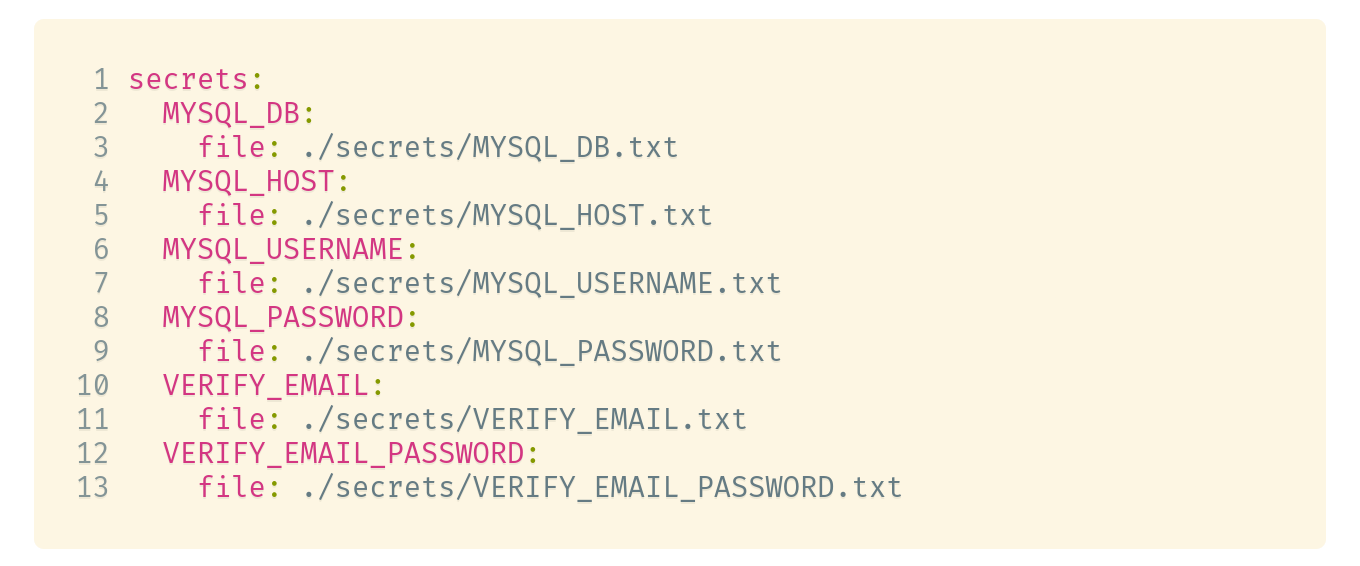
\includegraphics[width=1\textwidth]{images/Backend/secrets.png}
        \vspace{-25pt}
        \caption{Sokkas Docker Secrets in der \lstinline{docker-compose.yml}}
    \end{center}
\end{code}

\section{REST-API}

Damit die App und die Website auf die Daten der Datenbank zugreifen können, stellt der Server sogenannte Rest-Routes zur Verfügung. Jeder Computer mit Internetzugang kann auf diese Routes zugreifen insofern, die Richtigen HTTPs Anfragen an den Server gesendet werden.

Eine vollständige Dokumentation alles Rest-Routes befindet sich im Kapitel Rest-Routes-Dokumentation


\subsection{Bilder}

Bei \textbf{Skate-Buddy} erhalten sowohl die Skateparks, sowohl als auch ihre Obstacle Bilder. Um diese

\subsection{Verifikation}
\label{verification}

Bei der Registrierung müssen Nutzer ihre E-Mail-Adresse angeben. Um sicherzugehen, dass diese Adresse auch wirklich gültig ist, wurde mit Hilfe der Library \textit{nodemailer} ein simples E-Mail-Verifikationssystem implementiert. Ein Nutzer kann erst Bestellungen tätigen, wenn sein Nutzerkonto verifiziert ist.

Schon beim Start des Servers wird geprüft, ob die in den \textit{\nameref{dockersecrets}} gespeicherten Informationen zur Anmeldung bei Google-Mail korrekt sind (\lstinline{VERIFY_EMAIL} und \lstinline{VERIFY_EMAIL_PASSWORD}). \lstinline{VERIFY_EMAIL_PASSWORD} ist hier allerdings nicht wirklich das Passwort für das Google-Mail-Konto, sondern ein generiertes App-Passwort (myaccount.google.com/u/1/apppasswords).

Sofern die gespeicherten Anmeldedaten korrekt sind (und der Anmeldevorgang bei Google erfolgreich war), kann der Server vollautomatisch E-Mails an neue Nutzer versenden.

Wenn sich ein neuer Nutzer durch die REST-Route \textit{\nameref{usercreate}} mit einer laut RFC 5322 gültigen E-Mail-Adresse registriert, werden 64 zufällige Bytes generiert, welche anschließend in Base64 enkodiert werden und der entstandene String in Verbindung mit der ID des Nutzerkontos in einer Tabelle abgelegt wird.

Im selben Moment wird an die angegebene E-Mail-Adresse eine Nachricht mit einer URL gesendet, welche den generierten String enthält.

\begin{figure}[htp]
    \begin{center}
        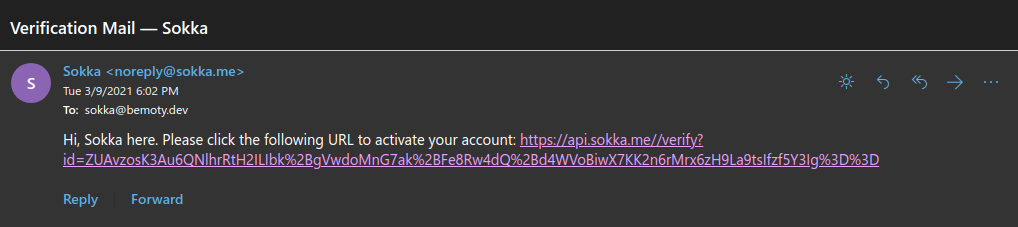
\includegraphics[width=1\textwidth]{images/Backend/mail.png}
        \caption{Eine E-Mail, welche durch Sokka bei der Verifizierung gesendet wurde}
    \end{center}
\end{figure}

Die URL in der E-Mail führt zur REST-Route \textit{\nameref{verify}}, welche, wenn der String in der URL gültig ist, das damit verbundene Nutzerkonto verifiziert.

\part{Theoretische Grundlagen}

\part{Theoretische Grundlagen}

\part{Theoretische Grundlagen}

\input{parts/2-theorie/1-programmiersprachen/index.tex}
\input{parts/2-theorie/2-haupttechnologien/index.tex}
\part{Theoretische Grundlagen}

\input{parts/2-theorie/1-programmiersprachen/index.tex}
\input{parts/2-theorie/2-haupttechnologien/index.tex}
\part{Theoretische Grundlagen}

\part{Theoretische Grundlagen}

\input{parts/2-theorie/1-programmiersprachen/index.tex}
\input{parts/2-theorie/2-haupttechnologien/index.tex}
\part{Theoretische Grundlagen}

\input{parts/2-theorie/1-programmiersprachen/index.tex}
\input{parts/2-theorie/2-haupttechnologien/index.tex}